\section{Quiz}

This remainder of this homework is a series of multiple choice questions related to the word2vec algorithm.

{\bf How to submit:}  Even though these are not coding questions, you will submit your response to
each question in the |src-quiz/submission.py| file.  This file will act as
your 'bubble sheet' for multiple choice questions in this course.  A sample response
might look like this:

\begin{center}
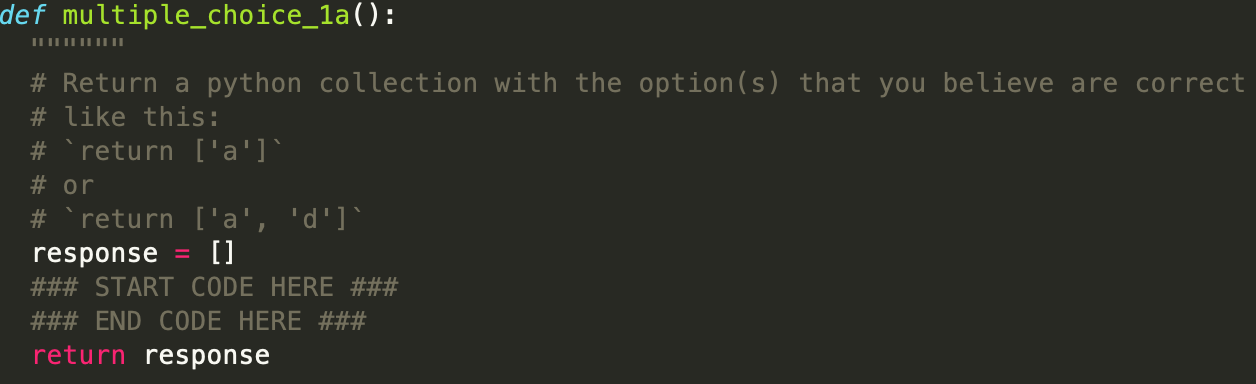
\includegraphics[width=1\textwidth]{sample_question_empty.png}
\end{center}

If you believe that |a| and |b| are the correct responses to this question, you
will type |response = [`a', `b']| between the indicated lines like this:

\begin{center}
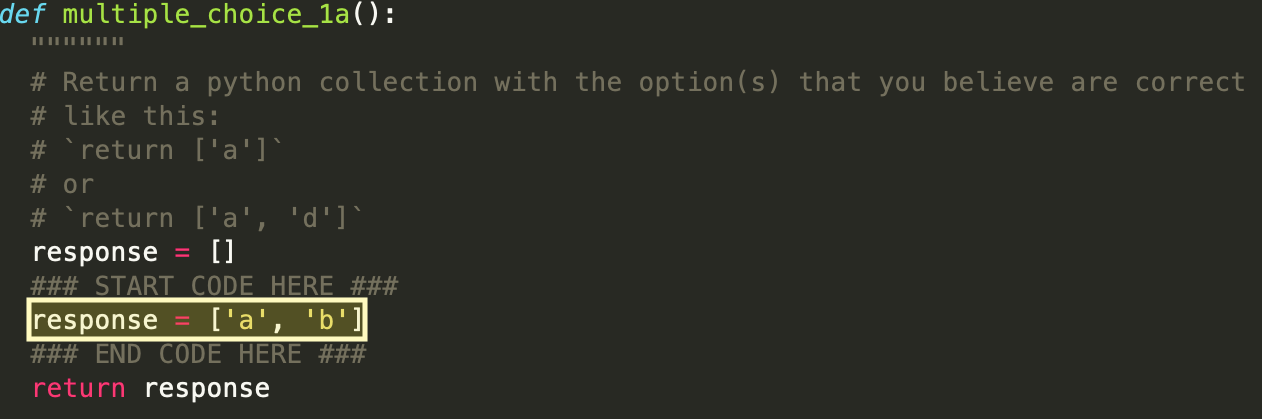
\includegraphics[width=1\textwidth]{sample_question_complete.png}
\end{center}

{\bf How to verify your submission:}
You can run the student version of the autograder locally like all coding
problem sets.  In the case of this problem set, the helper tests will verify
that your responses are within the set of possible choices for each question
(e.g. the helper functions will flag if you forget to answer a question of if
you respond with |[`a', `d']| when the choices are |[`a', `b', `c']|.)  See the
front pages of this assignment for instructions to run the autograder.
\clearpage

\begin{enumerate}[1.]
\item \points{quiz1}

{\em {\bf Note:}} For Question 1, reference the Python file |nmt_model.py| in your Assignment 4 coding files folder. 

The |generate_sent_masks()| function in |nmt_model.py| produces a tensor called |enc_masks|. It has a shape (batch size, max source sentence length) and contains 1s in positions corresponding to |pad| tokens in the input, and 0s for non-|pad| tokens. Look at how the masks are used during the attention computation in the |step()| function (lines 265-364). Which among the following options do you think explains why the masks are required? {\em{\bf Select all that apply}}.

\begin{enumerate}[(a)]
\item The masks are used to set the attention scores $e_{t,i}$ to $-\inf$ for all the positions $i$ that correspond to |pad| tokens in the source sentence. This means the encoder hidden states $h_i^\text{enc}$ that correspond to |pad| tokens have no effect on the attention output $a_t$.
\item The masks are used to set the attention scores $e_{t,i}$ to 0 for all the positions $i$ that correspond to |pad| tokens in the source sentence. This means the encoder hidden states $h_i^\text{enc}$ that correspond to |pad| tokens have no effect on the attention output $a_t$.
\item It is necessary to apply the masks to ensure we don’t apply attention on the encoder hidden states that correspond to |pad| tokens. 
\end{enumerate}

% ### START CODE HERE ###
% ### END CODE HERE ###

\item \points{quiz2}

The example below contains a Cherokee source sentence, reference English translation, NMT English translation, and error type. Choose the options that articulate a viable {\bf reason(s)} for the observed error that you might explore further. {\bf {\em Select all that apply.}}

{\bf Source Sentence:} {\em Yona utsesdo ustiyegv anitsilvsgi digvtanv uwoduisdei.}
\newline
{\bf Reference Translation:} {\em Fern had a crown of daises in her hair.}
\newline
{\bf NMT Translation:} {\em Fern had her hair with her hair.}
\newline
{\bf Error:} Repetition (`her hair')
\newline

\begin{enumerate}[(a)]
\item A possible reason is that the model attended to {\bf {\em hair}} twice, thus producing both mentions of {\bf {\em hair}} in the sentence.
\item The reference translation says {\bf {\em crown of daises}}, where the word {\bf {\em crown}} has no direct counterpart in the source sentence. These types of cases can be difficult for ``sequence-to-sequence + attention'' systems to produce.
\item Repetition can be a problem with the decoding algorithm (e.g. greedy decoding / beam search).
\end{enumerate}

% ### START CODE HERE ###
% ### END CODE HERE ###

\item
The examples below contain a Spanish source sentence, reference English translation, NMT English translation, and error type. For each example, analyze the error and choose the options that represent reasonable approaches to try to fix the error observed. {\bf {\em Select all that apply.}}

\begin{enumerate}[3a.]
\item \points{quiz3a}

{\bf Source Sentence:} {\em Un amigo me hizo eso -- Richard \underline{Bolingbroke}}
\newline
{\bf Reference Translation:} {\em A friend of mine did that -- Richard \underline{Bolingbroke}}
\newline
{\bf NMT Translation:} {\em A friend of mine did that -- Richard $\langle unk \rangle$}
\newline 
{\bf Error:} Out of vocabulary words ($\langle unk \rangle$)
\newline

\begin{enumerate}[(a)]
\item We could add a neural copy/pointer mechanism to copy words from the source sentence (e.g., names).
\item We could initialize the decoder part with weights of pre-trained language models (trained on a large English corpus) instead of initializing them with random weights.
\item We could switch to a subword-based NMT model (e.g. one using characters, BPE or word-pieces); this would enable the decoder to produce new (out-of-vocabulary) words.
\end{enumerate}

% ### START CODE HERE ###
% ### END CODE HERE ###

\item \points{quiz3b}

{\bf Source Sentence:} {\em Eso es mas de 100,000 hectareas.}
\newline
{\bf Reference Translation:} {\em That's more than 250 thousand acres.}
\newline
{\bf NMT Translation:} {\em That's over 100,000 acres.}
\newline
{\bf Error:} Incorrect numeric conversions (100,000 hectares = 250,000 acres, not 100,000 acres)
\newline
\href{https://www.unitconverters.net/area/acres-to-hectare.htm}{Acre and Hectare numeric conversions.}

\begin{enumerate}[(a)]
\item We could collect more Spanish to English translation pairs that contain examples with metric to imperial conversions.
\item We could supply the NMT system with a knowledge base of units of measurement and their conversion rates, and train a system to convert from metric to imperial (imagine such a system already exists outside of NMT, as a post-processing step).
\item We could implement a subword based NMT model (e.g. one using characters, BPE or word-pieces).
\end{enumerate}

% ### START CODE HERE ###
% ### END CODE HERE ###

\end{enumerate}

\item 

BLEU score is the most commonly used automatic evaluation metric for NMT systems. It is usually calculated across the entire test set, but here we will consider BLEU defined for a single example Suppose we have a source sentence $s$, a set of $k$ reference translations $r_1,....,r_k$ and a candidate translation $c$. To compute the BLEU score of $c$, we first compute the {\em modified n-gram precision} $p_n$ of $b_c$, for each of $n = 1, 2, 3, 4$:

\begin{equation*}
p_n = \frac{ \displaystyle \sum_{\text{ngram} \in c} \min \bigg( \max_{i=1,\dots,k} \text{Count}_{r_i}(\text{ngram}), \enspace \text{Count}_{c}(\text{ngram}) \bigg) }{\displaystyle \sum_{\text{ngram}\in c} \text{Count}_{c}(\text{ngram})}
\end{equation*}

Here, for each of the {\em n-grams} that appear in the candidate translation $c$, we count the maximum number of times it appears in any one reference translation, capped by the number of times it appears in $c$ (this is the numerator). We divide this by the number of {\em n-grams} in $c$ (denominator).

Next, we compute the {\em brevity penalty} {\bf BP}. Let $c$ be the length of $c$ and let $r*$ be the length of the reference translation that is closest to $c$ (in the case of two equally-close reference translation lengths, choose $r*$ as the shorter one)
\begin{equation*}
    BP = 
    \begin{cases}
        1 & \text{if } c \ge r^* \\
        \exp \big( 1 - \frac{r^*}{c} \big) & \text{otherwise}
    \end{cases}
\end{equation*}

Lastly, the BLEU score for candidate $c$ with respect to $r_1,...,r_k$ is:

\begin{align}
BLEU = BP \times \exp \Big( \sum_{n=1}^4 \lambda_n \log p_n \Big)
\end{align}

where $\lambda_1$, $\lambda_2$, $\lambda_3$, $\lambda_4$ are weights that sum to 1.

\begin{enumerate}[4a.]
\item \points{quiz4a}
Consider this example:

{\bf Source Sentence $s$:} el amor todo lo puede 
\newline
{\bf Reference Translation $r_1$:} love can always find a way
\newline
{\bf Reference Translation $r_2$:} love makes anything possible
\newline
{\bf NMT Translation $c_1$:} the love can always do
\newline
{\bf NMT Translation $c_2$:} love can make anything possible
\newline

Compute the BLEU scores for $c_1$ and $c_2$. Let $\lambda_i=0.5$ for $i \in {1 ,2}$ and $\lambda_i=0$ for $i \in {3 ,4}$ ({\bf this means we ignore 3-grams and 4-grams}, i.e., don't compute $p_3$ or $p_4$). Which of the two NMT translations (among $c_1$ and $c_2$) is considered the better translation according to the BLEU Score?

\begin{enumerate}[(a)]
\item $c_1$ has a higher BLEU score than $c_2$
\item $c_2$ has a higher BLEU score than $c_1$
\item Both translations, $c_1$ and $c_2$ are equally good
\end{enumerate}

% ### START CODE HERE ###
% ### END CODE HERE ###

\item \points{quiz4b}

The hard drive was corrupted and we lost Reference Translation $r_2$. Recompute BLEU scores for $c_1$ and $c_2$, this time with respect to $r_1$ only. Which of the two NMT translations has a higher BLEU Score?

\begin{enumerate}[(a)]
\item $c_1$ has a higher BLEU score than $c_2$
\item $c_2$ has a higher BLEU score than $c_1$
\item Both translations, $c_1$ and $c_2$ are equally good
\end{enumerate}

% ### START CODE HERE ###
% ### END CODE HERE ###

{\bf Footnote for Q4.1 and Q4.2}
{\em Why are multiple reference translations required?
\begin{itemize}
\item Often, there are many valid ways to translate a source sentence. This is particularly true for idiomatic phrases such as the above example. The BLEU metric is designed to accommodate this flexibility: an n-gram in c is rewarded if it appears in any one of the reference translations.
\item If we have multiple reference translations, the BLEU metric will thus reward similarity to any of the several valid translations.
\end{itemize}}

\item \points{quiz4c}

Which of the below statements are true regarding the BLEU scoring metric?

\begin{enumerate}[(a)]
\item BLEU can be calculated programmatically and is therefore fast to compute relative to human evaluation.
\item BLEU is based on absolute n-gram matching, so it doesn't reward synonyms, paraphrases, or different inflections of the same word.
\item BLEU uses multiple reference translations and hence does a better job than a human evaluator (assuming the evaluators are bilingual and do not use reference translations).
\end{enumerate}

% ### START CODE HERE ###
% ### END CODE HERE ###

\end{enumerate}

\item

In the lectures you learned about dot product attention, multiplicative attention, and additive attention. As a reminder, dot product attention is $e_{t,i} = s_t h_i^\intercal$, multiplicative attention is $e_{t,i} = s_t^\intercal W h_i$, and additive attention is $e_{t,i} = v^\intercal \tanh(W_1 h_i + W_2 s_t)$  ($v$, $W$, $W_1$ and $W_2$ are weights to be learned).
\begin{enumerate}[5a.]
\item \points{quiz5a}

Choose all options that accurately describe Dot Product attention:

\begin{enumerate}[(a)]
\item Encoder and decoder hidden states can be of different dimensions.
\item Requires additional weights in the model.
\item More computationally efficient compared to multiplicative and additive attention mechanisms.
\end{enumerate}

% ### START CODE HERE ###
% ### END CODE HERE ###

\item \points{quiz5b}

Choose all options that accurately describe Additive attention:

\begin{enumerate}[(a))]
\item Encoder and decoder hidden states can be of different dimensions.
\item Requires additional weights in the model.
\item More computationally efficient compared to multiplicative attention mechanisms.
\end{enumerate}

% ### START CODE HERE ###
% ### END CODE HERE ###

\item \points{quiz5c}

Choose all options that accurately describe Multiplicative attention:

\begin{enumerate}[(a)]
\item Encoder and decoder hidden states can be of different dimensions.
\item Requires additional weights in the model.
\item More computationally efficient compared to additive attention mechanisms.
\end{enumerate}

% ### START CODE HERE ###
% ### END CODE HERE ###
\end{enumerate}
\end{enumerate}